\section{Software de monitoração de SBCs}

\begin{frame}
\frametitle{Software de monitoração de SBCs}
\framesubtitle{Resumo}

\begin{itemize}
  \item Monitora todas as \textit{SBCs} do sistema de controle.
  \vspace{12pt}
  \item	Se comunica com um \textit{daemon} instalado em cada SBC.
  \vspace{12pt}
  \item Programa \textit{single-threaded}.
  \vspace{12pt}
  \item Implementação proposta:
  \begin{itemize}
    \item \textit{Threads} individuais para \textit{ìnterface}, \textit{rede} e
    processamento.
    \item Envio de comandos \textit{bash} aos SBCs selecionados.
    \item Interface gráfica: \textit{Qt}
  \end{itemize}
\end{itemize}

\end{frame}

\begin{frame}
\frametitle{Software de monitoração de SBCs}
\framesubtitle{Resumo}

\begin{figure}[h]

    \centering
    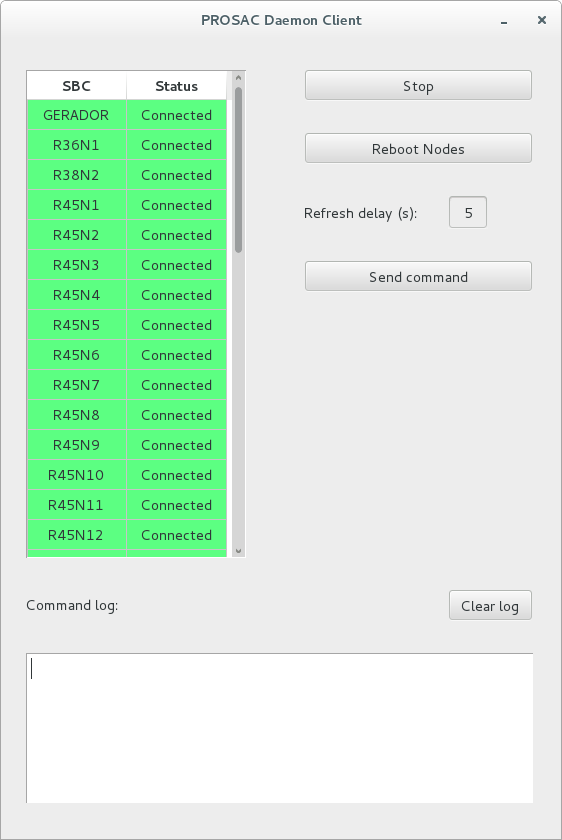
\includegraphics[height=0.7\textheight]{image/sbc}
    \caption {Interface gráfica de monitoramento de SBCs.}
    \label{fig:sbcs}
\end{figure}

\end{frame}